\documentclass[11pt,letter]{article}
\usepackage[top=1.00in, bottom=1.0in, left=1.1in, right=1.1in]{geometry}
\renewcommand{\baselinestretch}{1.1}
\usepackage[
singlelinecheck=false % <-- important
]{caption}
\usepackage{hyperref}%helps with the email address 
\usepackage{graphicx} %including pictrures

\def\labelitemi{--}
\parindent=0pt

\def\labelitemi{--}
\parindent=0pt

\newenvironment{smitemize}{
\begin{itemize}
  \setlength{\itemsep}{0pt}
  \setlength{\parskip}{0.8pt}
  \setlength{\parsep}{0pt}}
{\end{itemize}
}

\graphicspath{ {photosLatex/} }

\begin{document}
\bibliographystyle{/Users/Lizzie/Documents/EndnoteRelated/Bibtex/styles/besjournals}
\renewcommand{\refname}{\CHead{}}

\title{Directions to the vineyards:}
\date{ }
\maketitle

{\bf Quails' Gate: Main Estate vineyards} \\
Easy to find using Google Maps if you use the Quails' Gate Wineshop as the destination. 
From BC-97 North, turn right onto Gellatly Rd then left on Boucherie Rd. Quails' Gate Wineshop is about 5.5 km up the road. The parking lot for the main vineyard is a little bit before the Wineshop and is labelled with a "Staff Parking Only" sign. You can park here for the upper and lower vineyards (just across the road). We do not drive in the estate vineyards.

\begin{figure} [h]
  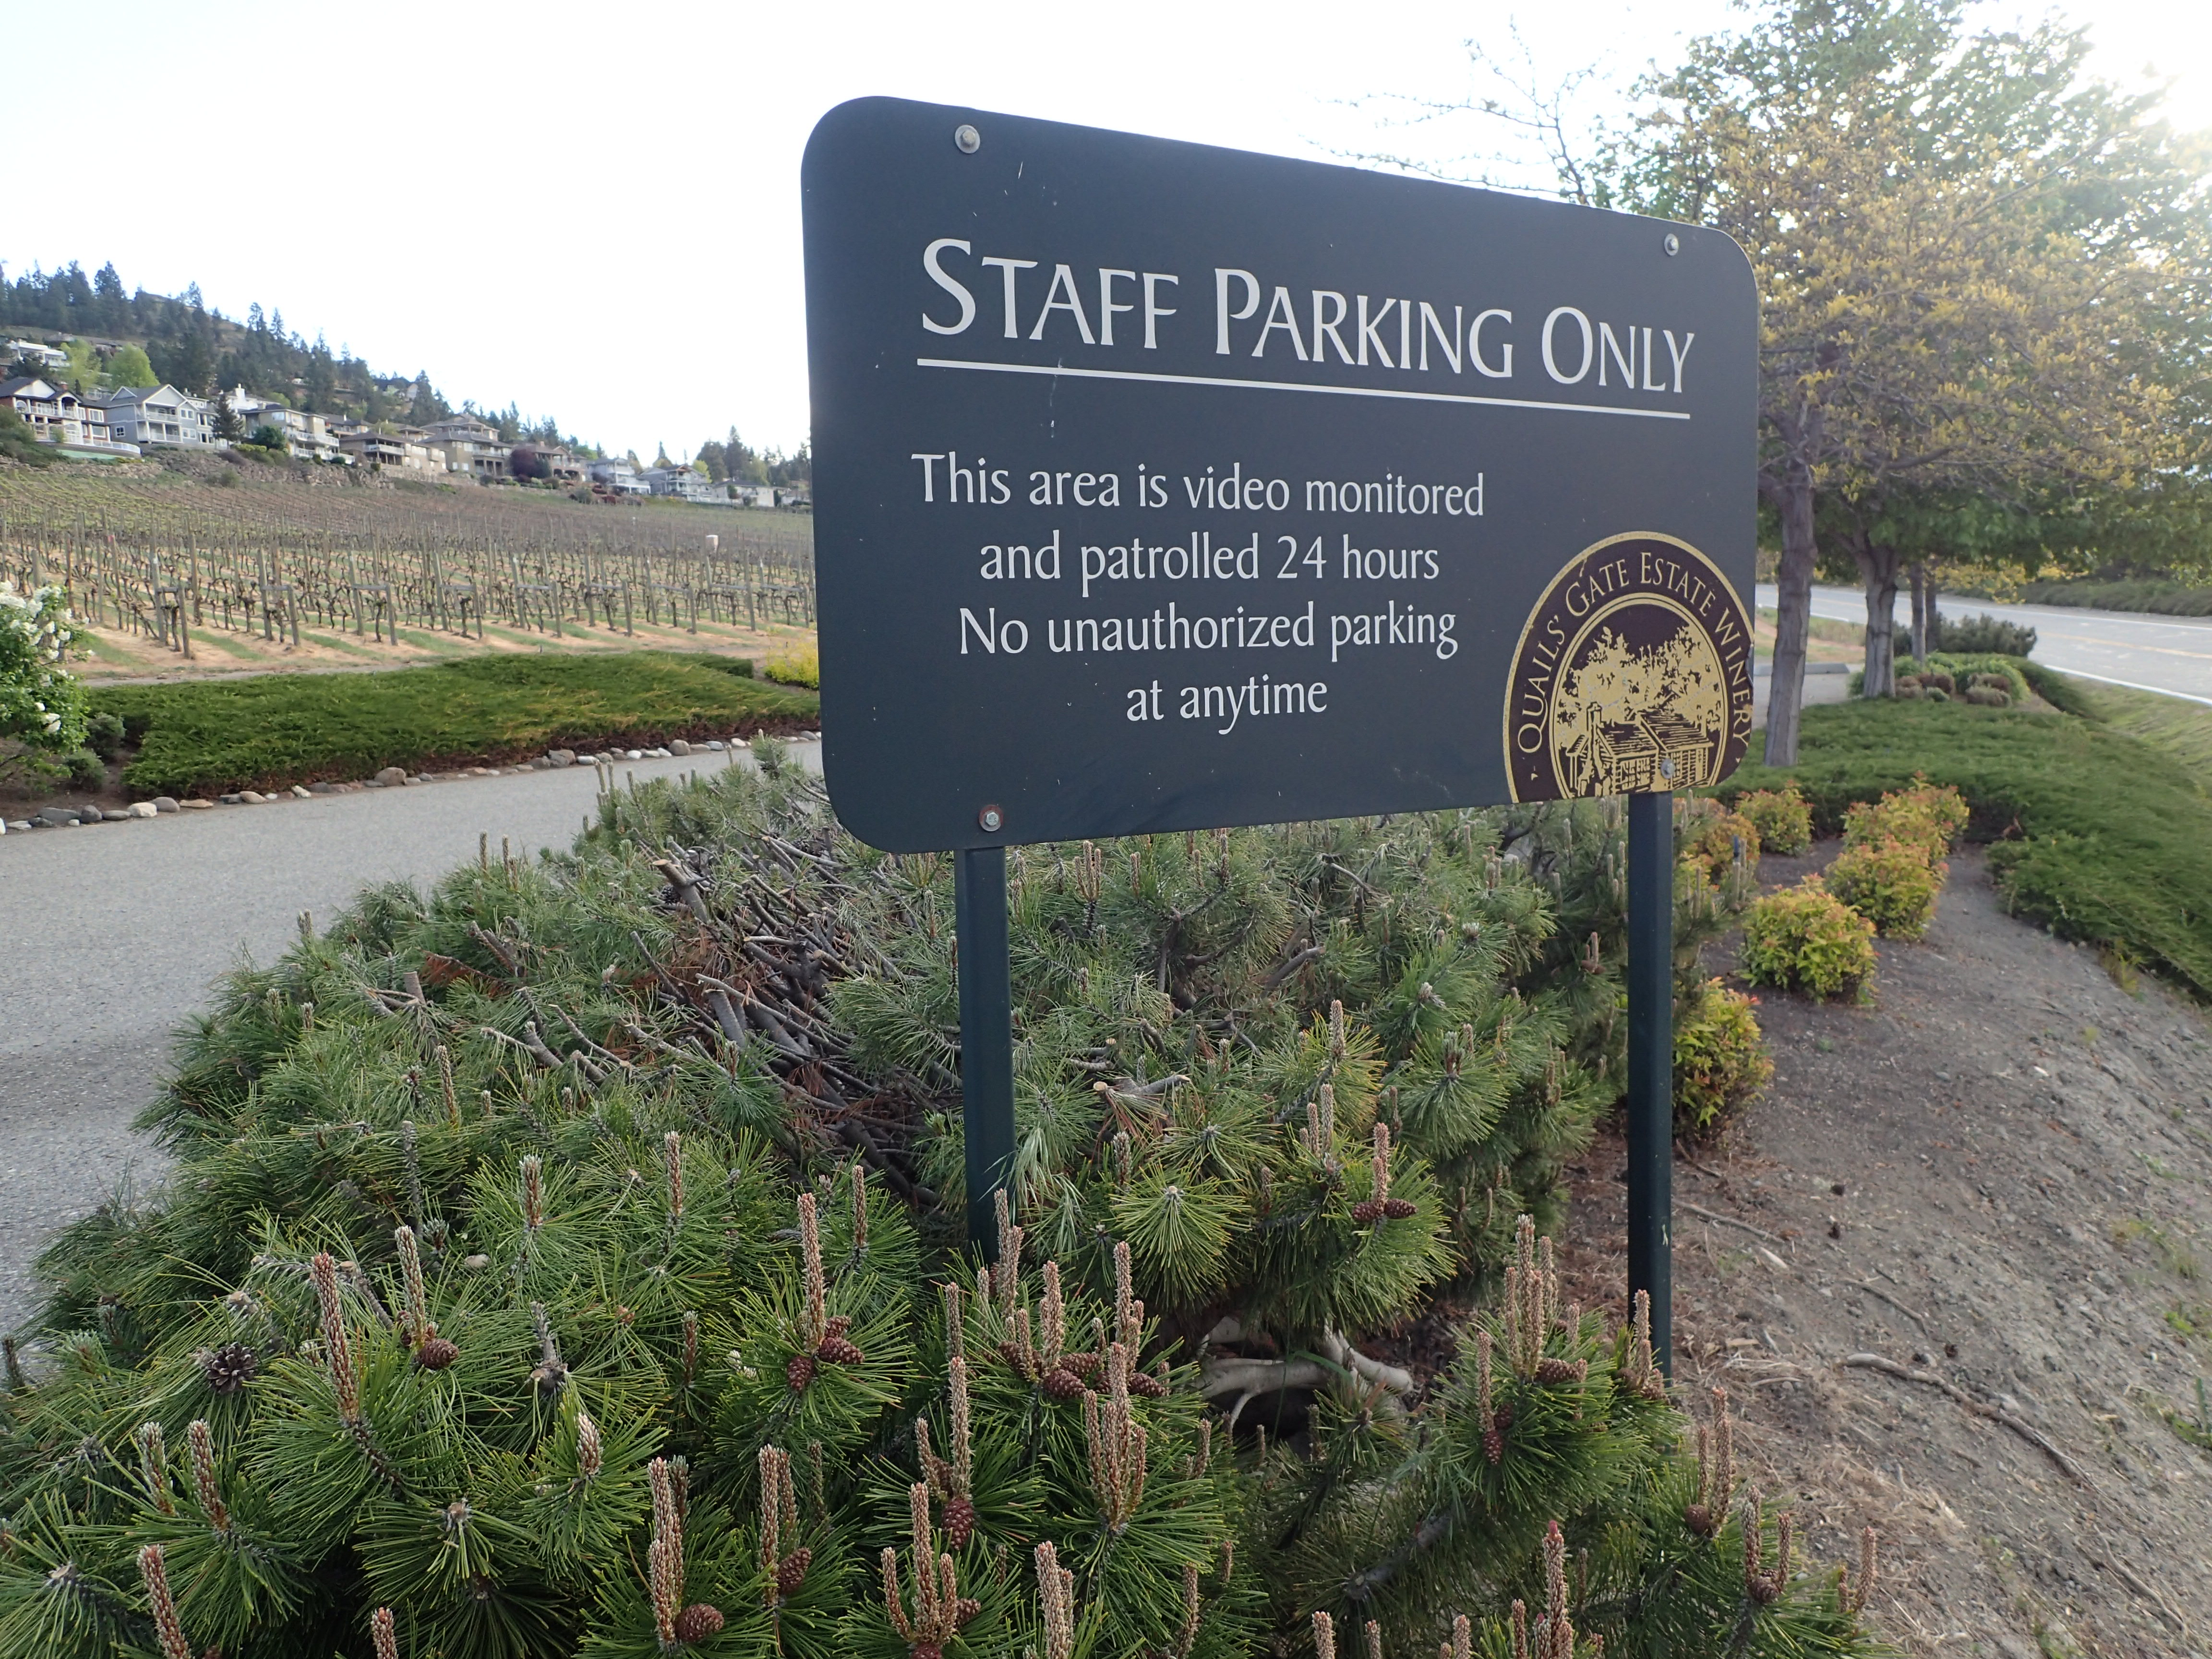
\includegraphics[scale = .25]{qgParkingLot.JPG}
  \caption{The sign marking the vineyard parking lot }
  \label{fig:QGparkingLot}
\end{figure}

There is no gate to the parking lot and no gate to prevent people from walking through the vineyard so as long as you have permission from Judy Wanbon to be in the vineyard, access at any time is easy. \\

{\bf Quails' Gate: Mannhardt Vineyard} \\
Mannhardt Vineyard is close to Quails' Gate. From Boucherie Rd, turn right on to Sunnyside Rd (turn is just after the Wineshop parking lot), left at the stop sign to Kelly Dr, and right at Aubrey Rd. Turning right on Aubrey essentially takes you into the vineyard. We have been driving around this vineyard.

Mannhardt does not seem to be gated. Technically, there is a gate but it has never been closed when we are there and non-vineyard people often walk through the site. You should only need permission from Judy and should be able to access it at any time. \\

{\bf Arterra: NK'MIP Cellars} \\
Easy to find using Google Maps if you set NK'MIP Cellars as the destination.
From BC-97 South, turn left on BC-3 E/Main Street and left onto 45 St. The 45 St corner has a Petro-Canada and a sign for NK'MIP Resort. Follow this road up to the resort and once in the resort parking lot, turn right and follow the road passed the sculpture of the turtle and man to the parking lot on the left. Across the road you should see the NK'MIP Cellars building and a garage/equipment shed. 

One section of the vineyard is at along the parking lot. The main vineyard is across the road - the gate is between the winery building and equipment shed. There is an additional gate from the resort parking lot that is obvious and decorative. I think it is best to use the other gates if possible. The spray board is on the equipment shed.

Mike Watson gave us a key that opened both gates to be returned at the end of the season. Get permission from Nelson Dutra to be in the vineyard. \\

{\bf Arterra: Dark Horse} \\
Easy to find with Google Maps if you set the destination to 4859 Mariposa Rd, Okanagan-Similkameen C, BC.
From BC-97 South, turn right onto Rd 11 then left on Mariposa Rd. You should see the main office building and parking lot behind a hedge right after the turn. Across the road from the parking lot are blocks 1 and 2. Driving around these will take you to an exit at the intersection of Mariposa Rd and Rd 11.

Following the paved road passed the office will take you up the hill to the other blocks. There is a sign marking Dark Horse. The spray board is on the side of the equipment shed.

I do not think the vineyard itself is gated - it has always been open when we arrive if it is. We will check this next time we are there. Get permission from Mike Watson but always check the spray board before starting work. \\

{\bf Arterra: Whitetail} \\
Can use 34401 Black Sage Rd, Oliver, BC V0H 1T0 to search on Google Maps.
From BC-97 South, turn left on Tucelnuit Dr (Jackson Triggs winery is on the corner) continue until the road ends at McKinney Rd. Turn left on McKinney Rd and a quick right to Black Sage Rd (you are essentially going straight but you have to change streets). Follow Black Sage Rd until you see the sign for Whitetail. 

You will enter into the main vineyard where you will find blocks C and D. There is another part of the vineyard with block B to the north, just across an empty field. If you follow the road to the hill, there is a road up the hill to block J on the top of the bench. To reach block F, you have to exit the main vineyard - turn left onto Black Sage Rd and take the first right onto Nk'Mip Rd. The vineyard with block F is the first right on this road. There are multiple exits back onto Black Sage Rd.

Get permission to be in the vineyard from Scott Carlson - he will tell you when they have sprayed. There should also be a spray board on the office according to Mike Watson. \\

{\bf Arterra: McIntyre} \\
Can use 4181-4101 McKinney Rd, Oliver, BC V0H 1T0 to search on Google Maps.
From BC-97 South, turn left on Tucelnuit Dr (Jackson Triggs winery is on the corner) continue until the road ends at McKinney Rd. Turn left onto McKinney Rd and follow it for about 1 km until you see McIntyre vineyard on the left. You will have to drive up the hill to get to the vineyard. The office is on the opposite side of the vineyard.

There is another exit/entrance on Arrow Head Rd between blocks A and C. Turning right out of block C (left from A) will take you out to McKinney Rd where you take a left and drive passed the main entrance to return to Tucelnuit Dr.

Get permission to be in the vineyard from Scott Carlson - he will tell you when they have sprayed. There should also be a spray board on the office according to Mike Watson. \\


\end{document}